\chapter{معماری نمونه مطالعاتی تاکسی‌آنلاین \lr{Uber}}
\section{معماری میکرو‌سرویس دامنه‌گرا}
اوبر \LTRfootnote{Uber} دارای بیش از ۲۲۰۰ میکرو‌سرویس است\cite{microservice_uber} و وجود تعداد زیادی میکرو‌سرویس باعث پیدایش پیچیدگی زیادی در نگهداری این سرویس ها و توسعه سرویس‌های جدید می‌شود تا جایی که \lr{Uber} سعی کرد با تغییراتی در معماری میکرو‌سرویس، معماری میکروسرویس دامنه‌گرا\LTRfootnote{Domain-Oriented Microservice Architecture} را ارائه دهد؛ در معماری میکرو‌سرویس دامنه‌گرا سعی شده است تا با حفظ مزیت‌های معماری میکرو‌سرویس، از پیچیدگی کل سیستم کاسته شود.

در معماری میکروسرویس، سرویس‌ها با عملکرد محدود به یک حوزه بر روی یک شبکه مستقر می‌شوند و از طریق رابط های تعریف شده به درخواست‌های که به صورت \lr{Remote Procedure Call} ارسال می‌شوند پاسخ می‌دهند؛ اوبر به دلایل زیر در سال ۲۰۱۲ معماری خود را از \lr{monolithic} به \lr{micro-service} تغییر داد:
\begin{itemize}
\item
ریسک‌های دردسترس‌پذیری\LTRfootnote{Availability} : یک خطا در سیستم \lr{monolithic} می‌توانست منجر به از دست خارج‌شدن کل سیستم \lr{Uber} شود.
\item
استقرار\LTRfootnote{Deployment} های پرخطر و زمان‌بر
\item
تفکیک ضعیف نگرانی‌ها\LTRfootnote{Concerns} : با‌وجود یک پایگاه کد بزرگ تفکیک مرز میان منطق تجاری و مولفه‌ها در یک سیستم با رشد بسیار سریع به خوبی صورت نمی‌پذیرد.
\item
اجرای ناکارآمد : وجود مشکلاتی که به چندین تیم وابستگی دارد، سبب می‌شود تا کارایی در اجرا بسیار پایین باشد.
\end{itemize}

هر چند مهاجرت از سیستم با معماری \lr{monolithic} به \lr{microservice} در زمانی که اندازه شرکت اوبر به صد‌ها مهندس رسیده بود بسیاری از مشکلات را حل کرد، اما زمانی که تعداد میکرو‌سرویس‌ها افزایش یافت شرکت متوجه پیچیدگی روزافزون معماری میکروسرویس شد؛ به عنوان مثال گاهی نیاز است برای یافتن ریشه‌ی یک خطا چندین میکروسرویس از تیم‌های مختلف مورد بررسی قرار گیرند. همچنین وابستگی میان سرویس‌ها گاه سبب می‌شود تا تاخیر پاسخ یک سرویس دیگر قابل قبول نباشد.همان طور که از پیچیدگی شبکه \lr{Uber} در سال ۲۰۱۸ \ref{fig:microserice_network} مشخص است میکروسرویس ها شدیدا به یکدیگر وابسته هستند.
\begin{figure}[h]
\label{fig:microserice_network}
\centering
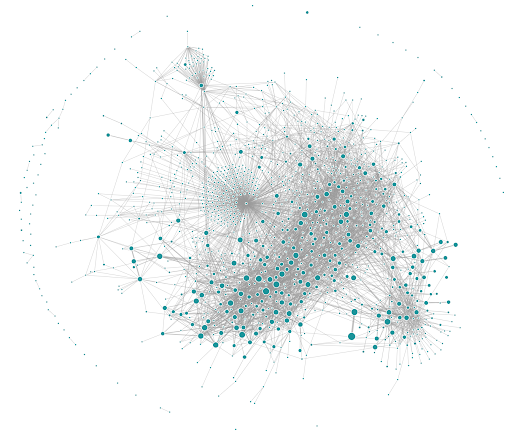
\includegraphics[width=8cm]{uber_service_network.png}
\end{figure}

به جهت پیاده‌سازی یک امکان جدید در \lr{Uber} یک تیم باید با سرویس‌‌های متفاوت متعلق به تیم‌های متفاوت کار کند و این عمل به جلسات زیادی بر روی طراحی و بازبینی کد نیاز دارد. همچنین مزیت معماری میکروسرویس در مورد داشتن خطوط مشخص مالکیت سرویس، هنگامی که تیم ها در سرویس های یکدیگر کد ایجاد می‌کنند، مدل‌های داده یکدیگر را اصلاح می کنند و حتی از طرف دارندگان سرویس نسخه‌های جدید را استقرار\LTRfootnote{deployment} می‌دهند، به خطر می افتد.در نتیجه با افزایش تعداد سرویس‌ها گویا با یک سیستم \lr{Network Monolithic} سر کار داریم که یکی از نتایج آن این است که چندین میکروسرویس به ظاهر مستقل نیاز دارند تا همزمان در سامانه مستقر شوند تا سامانه بدون نقص به عملکرد خود ادامه دهد.

در "معماری سرویس دامنه گرا" به طور عمده از روشهای تثبیت‌شده ساختار‌دهی کد مانند طراحی مبتنی بر دامنه \LTRfootnote{Domain-driven Design} \cite{evans2004domain}، معماری تمیز\LTRfootnote{Clean Architecture} \cite{martin2018clean}، معماری سرویس‌گرا\LTRfootnote{Service-Oriented Architecture} \cite{perrey2003service} و الگوهای طراحی شی‌گرا \LTRfootnote{object-oriented design} و رابطه گرا\LTRfootnote{interface-oriented design} استفاده می شود.










